\newpage
\bignumberedpart{Охорона праці}
    В даній дипломній роботі була розроблена система для визначення аномальної поведінки абонентів телефонної мережі.

    Користувачем системи визначення аномальної поведінки є розробник цієї системи, співробітники оператора мобільного зв'язку або спеціалісти із технічної підтримки, які віддалено налаштовують та впроваджують систему. В обов'язки цих людей входить робота із мультикомп'ютерною системою віддалено за допомогою комп'ютерної мережі зі свого робочого місця, що облаштовано персональним комп'ютером. Умови праці випливають із робочого місця працівника.

    В даній роботі досліджена організація пожежної та електричної безпеки, параметри приміщень та вплив шкідливих та небезпечних факторів на працівників.
    
\subsection{Характеристика приміщення}
\TBD
    План робочого приміщення приведений на рис.\ref{fig:lab-plan}.
    \begin{figure}[h!]
            \begin{center}
                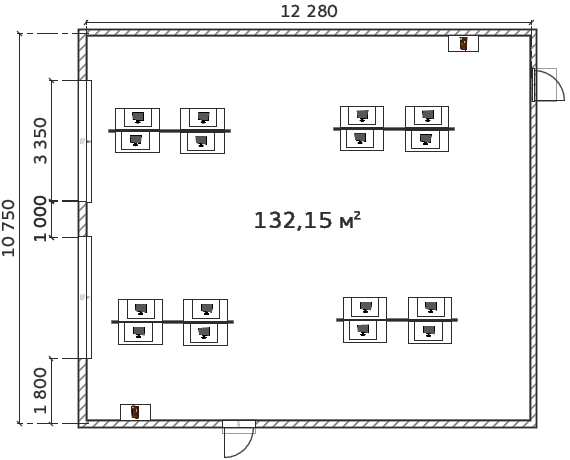
\includegraphics[scale=0.7]{labour/lab-plan}
            \end{center}
            \caption{Схема робочого приміщення}
            \label{fig:lab-plan}
    \end{figure}

    Геометричні параметри приміщення: ширина - 12.35 м, довжина - 10.6 м, висота - 3.5 м. Площа - 130.91 м кв., обєм - 458.2 м куб.
    Передбачається розміщення 16 робочих місць обладнаних системними блоками та рідкокристалічними моніторами.

    Згідно ДНАОП 0.00-1.31-99\cite{lab-dnaop} на одного працюючого повинно припадати не менше 6 м кв. площі та не менше 20 м. куб. oб'єму.
    У приведеному приміщенні 16 робочих місць і тоді відповідні параметри становлять 8.18 м. кв площі та при висоті стелі 3.5 м -  28.64 м куб. об'єму,
    що задовільняє норму.

    Для оздоблення слід використовувати матеріали з коефіцієнтом покриття для стелі 0.7 - 0.8, для стін 0.5 - 0.6.
    Покриття підлоги повинно бути матовим з коефіцієнтом відбиття 0.3 - 0.5. Поверхня підлоги повинна бути рівною і неслизькою.

\subsection{Небезпечні та шкідливі фактори}
    \subsubsection{Мікроклімат}
    Параметри мікроклімату визначаються з ДСН 3.3.6.042-99\cite{lab-dsn42}. Категорія робіт - легка Ia - роботи, що виконуються сидячи і не потребують
    важкого фізичного навантаження. Робоче місце постійне. Тому мікроклімат у робочому приміщенні повинен відповідати наступним вимогам.
    \begin{enumerate}
        \item оптимальна температура в холодний період року - 22..24С, у теплий - 23..25С;
        \item оптимальна відносна вологість 60-40\%;
        \item оптимальна швидкість руху повітря - 0.1 м/с.
    \end{enumerate}

    Для підтримки необхідної температури в холодний період року приміщення повинно бути облаштоване системою водяного центрального опалення з низьким тиском,
    а в теплий період року - системою кондиціонування -  спліт-система з внутрішнім блоком касетного типу.
    Так як вікна приміщення орієнтовані на схід, для уникнення перегрівання приміщення в літній період зранку, вікна повинні бути облаштовані жалюзями.

    \subsubsection{Освітлення}
    Освітлення у приміщенні здійснюється як за допомогою природних, так і за рахунок штучних джерел.
    Згідно ДБН В.2.5-28-2006\cite{lab-dbn28} сумарне освітлення робочої зони має бути таким, що сумарна освітленість на поверхні робочого столу становила 300-500 лк(для розряду зорових робіт Ia).

    Природнє освітлення здійснюється за рахунок вікон орієнтованих на схід, загальною площею 21 м кв.
    Штучне освітлення має здійснюватись переважно системою загального рівномірного освітлення -  люмінесцентними лампами типу ЛБ - 32 лампи
    ЛБ-18 G13 потужністю 18 Вт із застосуванням 8 світильників типу ЛВО(по 4 лампи) з зеркальними гратками.
    Система загального освітлення повинна становити лінії світильників, розташованих збоку від робочих місць, паралельно лінії зору працюючих.

    \subsubsection{Шум}
        Згідно ДСН 3.3.6.037-99\cite{lab-dsn37} рівень шуму та рівні звукового тиску для програмістів та вчених (творчі професії), мають бути не більше 50 дБA. 
        На робочому місці основними джерелами шуму є власний компютер та компьютери сусідів з еквівалентим рівнем шуму одного - 40 дБА, що в сумі дає 46 дБА
        і задовільняє норму.
        Еквівалентні рівні звукового тиску, що створює система кондиціонування повітря, повинні бути на 5 дБА менші.
    \subsubsection{Випромінювання}
    Рівні максимального електромагнітного випромінювання показані у таблиці\ref{tab:lab-waves}, причому максимальне значення
    електростатичного поля не повинно перевищувати 20 кВ/м.

    \begin{table}[h]
        \caption{Максимальні допустимі значення електромагнітного випромінювання на робочому місці}
        \begin{tabularx}{\textwidth}{| X | X | X |}
            \hline
            Напруженність & Електрична складова(В/м) & Магнітна складова(А/м) \\ \hline
            60 кГц до 3 мГц     & 50                       & 5                      \\ \hline
            3 кГц до 30 мГц     & 20                       & -                      \\ \hline
            30 кГц до 50 мГц    & 10                       & 0.3                    \\ \hline
            30 кГц до 300 мГц   & 5                        & -                      \\ \hline
        \end{tabularx}
        \label{tab:lab-waves}
    \end{table}

\subsection{Електробезпeка}
    Характер виконуваних у приміщенні робіт пов'язаний з постійним використанням електроустановок(системних блоків, моніторів), а тому необхідно забезпечити
    достатній рівень електробезпеки. Приміщення відноситься до класу без підвищеної небезпеки. Напруга у мережі становить 220В.

    Усі заземлені конструкції в приміщенні (батареї обігріву, водопровідні труби, кабелі з заземленим відкритим каналом),
    повинні бути захищені діелектричними щитками або сітками для недопущення потрапляння працівника під напругу. Для всієї проводки необхідно використовувати
    подвійну ізоляцію - основну та захисний короб.

    Необхідно забезпечити виконання наступних умов: усе обладнання в приміщенні повинно мати захист від короткого замикання та інших аварійних режимів,
    обладнання повинно підключатися виключно справними штепселями до стандартних електророзеток, лінія електромережі повинна бути окремою груповою трьохпроводною мережею, що складається
    з фазового, нульового робочого та нульового захисного провідників. Нульовий захисний провідник використовується для заземлення обладнання.


    \subsection{Пожежна безпека}
    Забезпечення пожежної безпеки у приміщенні повинно здійснюватися комплексом заходів: організаційних, системи виявлення пожеж та системи пожежогасіння.
    До пожежонебезпечних матеріалів у розглянутому приміщенні можна віднести - тверді горючі речовини(дерев'яні меблі - столи, шафи).
    Тоді згідно НАПБ Б.03.002-2007\cite{lab-napb} таке приміщення відноситься до категорії В(пожежонебезпечна).  Можливі пожежі - класу А(горіння твердих речовин), та класу Е - горіння електроустановок.

Приміщення повинно відповідати вимогам системи попередження пожеж (максимальне використання негорючих матеріалів, застосування аварійного відключення
на електроустановках, наявність систем виявлення пожежі, вогнегасників).
Так як основні причини пожежі у приміщенні пов'язані з електрикою(причому напруга не перевищує 380м), необхідно встановити автоматичну
дренчерну систему газового пожежогасіння з використанням хладона. Система повина бути обладнана димовими датчиками сповіщення про пожежу у кількості
не менше трьох.

\subsection{Техніка безпеки до виконання робіт}

    Роботи проводяться з використанням комп'ютера - пристрою, що працює під напругою. До виконання робіт допускаються виключно особи, що ознайомлені з усіма правилами безпеки.
    
    Перед початком робіт слід впевнитися, що робоче місце в порядку, а у приміщенні немає проблем з електрикою.
    Заборонено включати електроприбори, якщо на робочому місці присутня волога(наприклад, розлита вода).
    Якщо під час включення комп'ютера виникли іскри або дим, слід негайно виключити електричний рубильник,
    при необхідності скористатися вогнегасником, та сповістити про це спеціальні служби.
    Не слід самостійно переключати будь-які запчастини, переєднувати проводи - це повинен робити фахівець.
    При наявності відкритої проводки не слід розпочинати роботу.
    Не допускається наявність їжі та напоїв на робочому місці через загрози потрапляння води до електричних мереж.
